% Chapter 1

\chapter{Introduction to Wireless Sensor Networks} % Main chapter title
\label{Chapter1} % To reference to this chapter elsewhere, use \ref{Chapter1} 
\lhead{Chapter 1. \emph{Sound nomenclature}} % This is for the header on each page - perhaps a shortened title
%\textsf{\textsl{Written by Bjorn Deraeve}}
%----------------------------------------------------------------------------------------

\section{Introduction}
Sound is the human perception of little changes in air pressure. This oscillation of pressure, referred to as a sound wave, is a mechanical wave propagated through a solid, liquid or gas and is composed of frequencies within the range of hearing. For humans this is between about 20 Hz and 20 000 Hz, however the upper limit generally decreases with one's age.   The changes in pressure must also be big enough in order to be audible.

\begin{equation}
L_{P} = 10\cdot \mathrm{log}_{10} (\frac{p^{2}}{p_{ref^{2}}} ) = 20 \cdot \mathrm{log}_{10} (\frac{p}{p_{ref}}) \medspace dB
\end{equation}
where p is the rms value of the measured sound pressure and pref is the reference sound pressure, pref = 20 microPa (rms), considered as the threshold of human hearing.
%----------------------------------------------------------------------------------------

\section{Sound characteristics}
A sound is defined by several characteristics. The most important are pitch (dutch: 'toonhoogte'), timbre (dutch: 'klankkleur') and are briefly introduced in this section. Other characteristics are volume and the duration of the rising of the sound, of the persistence and of the damping.
%----------------------------------------------------------------------------------------

\subsection{Pitch and tone}
For the human ear a pure tone is a sound with a constant frequency and timbre. This 
%----------------------------------------------------------------------------------------

\subsection{Timbre}
Timbre is the quality of a sound that distinguishes different musical instruments and 

\subsubsection{Spectral diagram}
At this moment it is interesting to have a look at the spectral diagram of a sound. This  for the way air pressure changes with time but not for the actual timbre of a sound.
\begin{figure}[htbp]
\centering
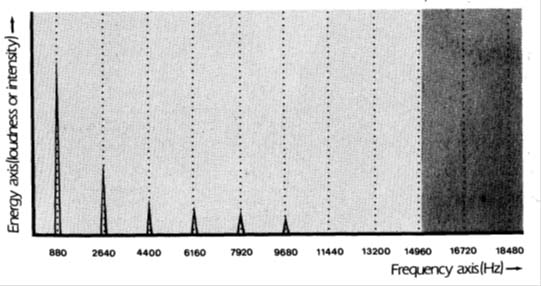
\includegraphics[height=5cm]{spectral}
\rule{30em}{0.5pt}
\caption{Spectral diagram of a timbre}
\label{fig:spectral}
\end{figure} \\
How can we interpret figure \ref{fig:spectral}? The line on the left is the fundamental  fundamental frequency (pitch). In other words: each complex sound can be resolved into mixtures of sine functions which may differ in amplitude and period but of which all periods are related as an integer multiple. This resolving into different components is called a Fourier transformation or analysis of the signal. \\ The spectrum as in figure \ref{fig:spectral} shows clearly the present frequencies (= partials, overtones or harmonics) and their energy level.
\begin{figure}[htbp]
   \centerline{\hbox{
   \epsfxsize=1.2in
   \epsffile{/fourier.jpg}
     }
  }
  \caption{Sketch of Fourier}
  \label{fig:fourier}
\end{figure}

